\documentclass{article}

\date{17 avril 2024}
\usepackage[nb-sem=2, auteurs={George Ober}]{../kholles}

\usepackage{tikz}
\usetikzlibrary{calc,trees,positioning,arrows,fit,shapes,calc}

\begin{document}

\maketitle

\begin{question_kholle}{Montrer qu'une composée d'applications inj/surj/bij est inj/surj/bij}
    Soient $u : E \to F$ et $v: F \to G$
    \begin{itemize}[label = $\lozenge$]
        \item Supposons $u$ et $v$ injectives.
        
        Soient $(x_{1}, x_{2}) \in E^{2}$ fq tels que $(v \circ u) (x_{1}) =(v\circ u)(x_{2})$.
        
        Alors $v(u(x_{1})) = v(u(x_{2}))$, mais $v$ est injective donc, $u(x_{1})= u(x_{2})$ mais $u$ est injective donc $x_{1} = x_{2}$.
        Ainsi $v \circ u$ est injective.
        \item Supposons $u$ et $v$ surjectives
        Soit $y \in G$ fixé quelconque.
        
        $v$ est surjective donc $\exists t \in F : v(t) = y$
        
        $u$ est surjective, donc $\exists x \in E : u(x) = t$
        Ainsi,
        $$
        (v \circ u) (x) = v(u(x)) = v(t) = y
        $$
        Donc $v \circ u$ est surjective.
        
        \item Supposons $u$ et $v$ bijectives.
        
        Le fait que $v \circ u$ est une bijection est une conséquence des deux points précédents.
        
    \end{itemize}
    
\end{question_kholle}
\begin{question_kholle}{Montrer que, si $u$ est une application de $E$ dans $F$, si $v$ est une application de $F$ dans $E$ telle que $v \circ u = \mathrm{Id}_E$ et $u \circ v = \mathrm{Id}_F$ alors $u$ est bijective ($v$ aussi) et sa bijection réciproque est $v$}
    Soient $(u, v) \in \mathcal{F}(E, F) \times \mathcal{F}(F, E)$ qui satisfont les conditions de l'énnoncé.
    \begin{itemize}[label=$\lozenge$]
        \item $u$ est injective
        
        Soient $(x_{1}, x_{2}) \in E^{2}$ fixés quelconques tels que $u(x_{1}) = u(x_{2})$. Alors $v(u(x_{1})) = v(u(x_{2}))$. Donc $x_{1} = x_{2}$ puisque $v \circ u = \mathrm{Id}_{E}$
        
        \item $u$ est surjective
        Soit $y \in F$ fixé quelconque. Posons $t = v(y)$. Ainsi, $u(t) = u(v(y))= y$ car $u \circ v = \mathrm{Id}_{F}$
        
        
    \end{itemize}
    Ainsi, $u$ est bijective, notons $u^{-1}$ sa bijection réciproque
    \begin{align*}
        u^{-1} \circ (u \circ v ) &= (u^{-1} \circ u) \circ v\\
        u^{-1} \circ \mathrm{Id}_{F} &= \mathrm{Id}_{E}\circ v\\
        u^{-1} &= v
    \end{align*}
    
\end{question_kholle}

\begin{question_kholle}{Montrer que $v \circ u$ injective implique $u$ injective + montrer que cela n'implique pas $v$ injective.}
    Soient $(u, v) \in \mathcal{F}(E, F) \times \mathcal{F}(F, G)$.
    
    Supposons $v \circ u$ est injective
    Soient $(x_1, x_2) \in E^2$ fixés quelconques tels que $u(x_1) = u(x_2)$.
    Composons par $v$ à gauche : $v \circ u ( x_1 ) = v \circ u (x_2)$
    Puisque $v \circ u$ est injective, cela implique que $x_1 = x_2$.
    
    
    \begin{figure}[!h]
        \centering
        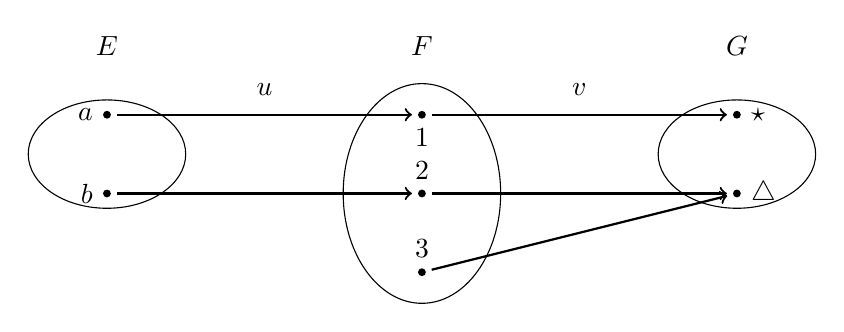
\begin{tikzpicture}[ele/.style={fill=black,circle,minimum width=.8pt,inner sep=1pt},every fit/.style={ellipse,draw,inner sep=-2pt}]
            \node[label=above:$E$] at (0, 4.5) {};
            \node[label=above:$F$] at (4, 4.5) {};
            \node[label=above:$G$] at (8, 4.5) {};
            
            \node[label=above:$u$] at (2, 4) {};
            \node[label=above:$v$] at (6, 4) {};
            
            
            \node[ele,label=left:$a$] (a1) at (0,4) {};    
            \node[ele,label=left:$b$] (a2) at (0,3) {};    
            
            \node[ele,,label=below:$1$] (b1) at (4,4) {};
            \node[ele,,label=above:$2$] (b2) at (4,3) {};
            \node[ele,,label=above:$3$] (b3) at (4,2) {};
            
            \node[ele,,label=right:$\star$] (c1) at (8,4) {};
            \node[ele,,label=right:$\triangle$] (c2) at (8,3) {};
            
            \node[draw,fit= (a1) (a2) ,minimum width=2cm] {} ;
            \node[draw,fit= (b1) (b2) (b3) ,minimum width=2cm] {} ;  
            \node[draw,fit= (c1) (c2) ,minimum width=2cm] {} ; 
            
            \draw[->,thick,shorten <=2pt,shorten >=2pt] (a1) -- (b1);
            \draw[->,thick,shorten <=2pt,shorten >=2] (a2) -- (b2);
            \draw[->,thick,shorten <=2pt,shorten >=2] (b1) -- (c1);
            \draw[->,thick,shorten <=2pt,shorten >=2] (b2) -- (c2);
            \draw[->,thick,shorten <=2pt,shorten >=2] (b3) -- (c2);
        \end{tikzpicture}
    \end{figure}
    Ici, $v \circ u$ est injective, on a montré que cela impliquait $u$ injective. Pourtant, $v$ n'est pas injective.
    
\end{question_kholle}

\begin{question_kholle}{Montrer que $v \circ u$ surjective implique $v$ surjective + montrer que cela n'implique pas $u$ surjective.}
    Soient $(u, v) \in \mathcal{F}(E, F) \times \mathcal{F}(F, G)$.
    
    Supposons $v \circ u$ est surjective
    Soit $y \in G$ fixé quelconque.
    Puisque $v \circ u$ est surjective, $\exists x \in E : (v \circ u)(x) = y$
    Donc $v(u(x)) = y$.
    Donc, en posant $t = u(x)$, on a $v(t) = y$.
    Ainsi, $v$ est surjective.
    
    \begin{figure}[!h]
        \centering
        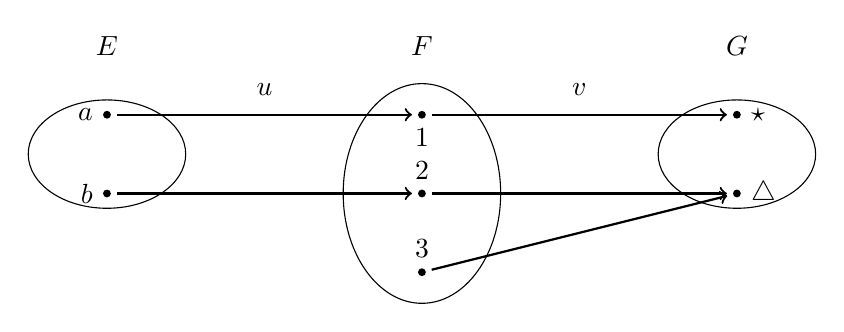
\begin{tikzpicture}[ele/.style={fill=black,circle,minimum width=.8pt,inner sep=1pt},every fit/.style={ellipse,draw,inner sep=-2pt}]
            \node[label=above:$E$] at (0, 4.5) {};
            \node[label=above:$F$] at (4, 4.5) {};
            \node[label=above:$G$] at (8, 4.5) {};
            
            \node[label=above:$u$] at (2, 4) {};
            \node[label=above:$v$] at (6, 4) {};
            
            
            \node[ele,label=left:$a$] (a1) at (0,4) {};    
            \node[ele,label=left:$b$] (a2) at (0,3) {};    
            
            \node[ele,,label=below:$1$] (b1) at (4,4) {};
            \node[ele,,label=above:$2$] (b2) at (4,3) {};
            \node[ele,,label=above:$3$] (b3) at (4,2) {};
            
            \node[ele,,label=right:$\star$] (c1) at (8,4) {};
            \node[ele,,label=right:$\triangle$] (c2) at (8,3) {};
            
            \node[draw,fit= (a1) (a2) ,minimum width=2cm] {} ;
            \node[draw,fit= (b1) (b2) (b3) ,minimum width=2cm] {} ;  
            \node[draw,fit= (c1) (c2) ,minimum width=2cm] {} ; 
            
            \draw[->,thick,shorten <=2pt,shorten >=2pt] (a1) -- (b1);
            \draw[->,thick,shorten <=2pt,shorten >=2] (a2) -- (b2);
            \draw[->,thick,shorten <=2pt,shorten >=2] (b1) -- (c1);
            \draw[->,thick,shorten <=2pt,shorten >=2] (b2) -- (c2);
            \draw[->,thick,shorten <=2pt,shorten >=2] (b3) -- (c2);
        \end{tikzpicture}
    \end{figure}
    
    Ici, $v \circ u$ est surjective, on a montré que cela impliquait $v$ surjective. Pourtant, $u$ n'est pas surjective. 
    
\end{question_kholle}

\textbf{Remarque} : Les deux contre contre-exemples exhibés ici sont les mêmes, mais il y en a bien d'autres où $v \circ u$ n'est pas bijective.

\begin{question_kholle}{Soit $u$ une application de $E$ dans $F$. Si $A$ et $A'$ sont des parties de $E$, y'a-t-il égalité entre $u(A \cap A')$ et $u(A) \cap u(A')$? (On justifiera les réponses aux deux inclusions suggérées par la question)}
    Soit $u \in \mathcal{F}(E, F)$ fixée quelconque, $(A, A') \in \mathcal{P}(E)^{2}$, deux parties de $E$.
    \begin{itemize}[label=$\lozenge$]
        \item Soit $y \in u(A \cap A')$ fixé quelconque.
        Par définition $\exists x \in (A \cap A') : u(x) = y$.
        Ainsi, $x \in A \implies u(x) \in u(A)$
        $x \in A' \implies u(x) \in u(A')$
        
        $$
        \left.
        \begin{array}{ll}
            u(x) \in u(A) \\
            u(x) \in u(A')
        \end{array}\right\} \implies u(x) \in u(A) \cap u(A')
        $$
        Donc $u(A \cap A') \subset u(A) \cap u(A')$.
        
        \item En revanche l'inclusion réciproque est fausse: considérons
        $$
        u \left|\begin{array}{ll} \{ 1, 2, 3, 4 \} &\to \{ a, b, c, d \} \\ 1 &\mapsto a \\
            2  & \mapsto b  \\
            3  & \mapsto a \\
            4  & \mapsto d\end{array}\right.
            $$
            Si on choisit $A = \{ 1, 2 \}$ et $A' = \{ 2, 3 \}$.
            
            Alors, $u(A) = \{ a, b \}$, et $u(A') = \{ a, b \}$
            $u(A \cap A') = u(\{ 2 \}) = \{ b \}$
            
            et $u(A) \cap u(A') = \{ a, b \} \not\subset \{  b \}$
        \end{itemize}
    \end{question_kholle}
    \begin{question_kholle}{Montrer que, si $u$ est une application de $E$ dans $F$. Si $B$ est une partie de $F$, alors $u^{-1}(F\setminus B) = E \setminus u^{-1}(B)$.}
        Soit $x \in u^{-1}(F\setminus B)$. Raisonnons par équivalences. 
        
        \begin{align*}
            x \in u^{-1}(F \setminus B) 
            & \iff u(x) \in F \setminus B \\
            & \iff \mathrm{non} (u(x) \in B) \\
            & \iff \mathrm{non} (x \in u^{-1}(B)) \\
            & \iff x \in E \setminus u^{-1}(B)
        \end{align*}
        
    \end{question_kholle}
    \begin{question_kholle}{Montrer que, parmi les entiers ne s'écrivant qu'avec des 7, il existe au moins un multiple de 61.}
        
        Posons $s$ la suite des entiers tels que $\forall n \in \mathbb{N}^{*}, s_{n} = \underbrace{ 7\dots 7 }_{ n \text{ fois} }$.
        Considérons les $62$ premiers termes de la suite.
        
        Puisqu'il y a $61$ classes de congruences modulo $61$, le principe des tiroirs de Dirichlet nous permet d'affirmer que $\exists (k, l) \in [ \! [ 1, 62 ] \!]^{2}, k < l:s_{k} \equiv s_{l}[61]$.
        
        Remarquons maintenant que $s_{l}-s_{k} \equiv 0 [61]$, autrement dit que $61\mid s_{l} - s_{k}$.
        
        Cependant, $$
        s_{l} - s_{k} = \underbrace{ 7\dots7 }_{ l \text{ fois} } - \underbrace{ 7 \dots 7 }_{ k \text{ fois} } = \underbrace{ 7 \dots 7 }_{ l-k \text{ fois} } \underbrace{ 0 \dots 0 }_{ k \text{ fois} } = s_{l-k} \times 10^{k}
        $$
        Donc $61 \mid 10^{k} \times s_{l-k}$, mais $\mathrm{pgcd}(61, 10^{k}) = 1$ donc le théorème de Gauss donne $61\mid s_{l-k}$.
        
        Ainsi, parmi les entiers ne s'écrivant qu'avec des 7, il existe au moins un multiple de 61.
    \end{question_kholle}
    \end{document}
    